\documentclass[11pt,compress,t,notes=noshow, xcolor=table]{beamer}
\usepackage[]{graphicx}\usepackage[]{color}
% maxwidth is the original width if it is less than linewidth
% otherwise use linewidth (to make sure the graphics do not exceed the margin)
\makeatletter
\def\maxwidth{ %
  \ifdim\Gin@nat@width>\linewidth
    \linewidth
  \else
    \Gin@nat@width
  \fi
}
\makeatother

\newcommand{\citebutton}[2]{%
\beamergotobutton{\href{#2}{#1}}%
}

\newcommand{\blu}[1]{\textcolor{blue}{#1}}
\newcommand{\org}[1]{\textcolor{orange}{#1}}
\newcommand{\ques}{\textbf{\textcolor{red}{Question:  }}}
\newcommand{\questionssofar}{\begin{frame}\frametitle{Any questions?}\end{frame}}

\newcommand\warning{%
 \makebox[1.4em][c]{%
 \makebox[0pt][c]{\raisebox{.1em}{\scriptsize!}}%
 \makebox[0pt][c]{\color{red}\normalsize$\bigtriangleup$}}}%

\definecolor{fgcolor}{rgb}{0.345, 0.345, 0.345}
\newcommand{\hlnum}[1]{\textcolor[rgb]{0.686,0.059,0.569}{#1}}%
\newcommand{\hlstr}[1]{\textcolor[rgb]{0.192,0.494,0.8}{#1}}%
\newcommand{\hlcom}[1]{\textcolor[rgb]{0.678,0.584,0.686}{\textit{#1}}}%
\newcommand{\hlopt}[1]{\textcolor[rgb]{0,0,0}{#1}}%
\newcommand{\hlstd}[1]{\textcolor[rgb]{0.345,0.345,0.345}{#1}}%
\newcommand{\hlkwa}[1]{\textcolor[rgb]{0.161,0.373,0.58}{\textbf{#1}}}%
\newcommand{\hlkwb}[1]{\textcolor[rgb]{0.69,0.353,0.396}{#1}}%
\newcommand{\hlkwc}[1]{\textcolor[rgb]{0.333,0.667,0.333}{#1}}%
\newcommand{\hlkwd}[1]{\textcolor[rgb]{0.737,0.353,0.396}{\textbf{#1}}}%
\let\hlipl\hlkwb

\usepackage{framed}
\makeatletter
\newenvironment{kframe}{%
 \def\at@end@of@kframe{}%
 \ifinner\ifhmode%
  \def\at@end@of@kframe{\end{minipage}}%
  \begin{minipage}{\columnwidth}%
 \fi\fi%
 \def\FrameCommand##1{\hskip\@totalleftmargin \hskip-\fboxsep
 \colorbox{shadecolor}{##1}\hskip-\fboxsep
     % There is no \\@totalrightmargin, so:
     \hskip-\linewidth \hskip-\@totalleftmargin \hskip\columnwidth}%
 \MakeFramed {\advance\hsize-\width
   \@totalleftmargin\z@ \linewidth\hsize
   \@setminipage}}%
 {\par\unskip\endMakeFramed%
 \at@end@of@kframe}
\makeatother

\definecolor{shadecolor}{rgb}{.97, .97, .97}
\definecolor{messagecolor}{rgb}{0, 0, 0}
\definecolor{warningcolor}{rgb}{1, 0, 1}
\definecolor{errorcolor}{rgb}{1, 0, 0}
\newenvironment{knitrout}{}{} % an empty environment to be redefined in TeX

\usepackage{alltt}
\newcommand{\SweaveOpts}[1]{}  % do not interfere with LaTeX
\newcommand{\SweaveInput}[1]{} % because they are not real TeX commands
\newcommand{\Sexpr}[1]{}       % will only be parsed by R
\newcommand{\xmark}{\ding{55}}%


\usepackage[english]{babel}
\usepackage[utf8]{inputenc}

\usepackage{dsfont}
\usepackage{verbatim}
\usepackage{amsmath}
\usepackage{amsfonts}
\usepackage{amssymb}
\usepackage{bm}
\usepackage{csquotes}
\usepackage{multirow}
\usepackage{longtable}
\usepackage{booktabs}
\usepackage{enumerate}
\usepackage[absolute,overlay]{textpos}
\usepackage{psfrag}
\usepackage{algorithm}
\usepackage{algpseudocode}
\usepackage{eqnarray}
\usepackage{arydshln}
\usepackage{tabularx}
\usepackage{placeins}
\usepackage{tikz}
\usepackage{setspace}
\usepackage{colortbl}
\usepackage{mathtools}
\usepackage{wrapfig}
\usepackage{bm}
\usepackage{amsmath}
\usepackage{pifont}

\usetikzlibrary{shapes.multipart,shapes,arrows,automata,positioning,calc,chains,trees, shadows}
\tikzset{
  %Define standard arrow tip
  >=stealth',
  %Define style for boxes
  punkt/.style={
    rectangle,
    rounded corners,
    draw=black, very thick,
    text width=6.5em,
    minimum height=2em,
    text centered},
  % Define arrow style
  pil/.style={
    ->,
    thick,
    shorten <=2pt,
    shorten >=2pt,}
}

\tikzstyle{vec}=[draw, rectangle, fill = white, minimum width=5mm, minimum height=1cm, inner sep = 2pt]

\usepackage{subfig}

% Defines macros and environments
\usepackage{../../style/lmu-lecture}


\let\code=\texttt
\let\proglang=\textsf

\setkeys{Gin}{width=0.9\textwidth}

\setbeamertemplate{frametitle}{\expandafter\uppercase\expandafter\insertframetitle}

\usepackage{bbm}
% basic latex stuff
\newcommand{\pkg}[1]{{\fontseries{b}\selectfont #1}} %fontstyle for R packages
\newcommand{\lz}{\vspace{0.5cm}} %vertical space
\newcommand{\dlz}{\vspace{1cm}} %double vertical space
\newcommand{\oneliner}[1] % Oneliner for important statements
{\begin{block}{}\begin{center}\begin{Large}#1\end{Large}\end{center}\end{block}}


%new environments
\newenvironment{vbframe}  %frame with breaks and verbatim
{
 \begin{frame}[containsverbatim,allowframebreaks]
}
{
\end{frame}
}

\newenvironment{vframe}  %frame with verbatim without breaks (to avoid numbering one slided frames)
{
 \begin{frame}[containsverbatim]
}
{
\end{frame}
}

\newenvironment{blocki}[1]   % itemize block
{
 \begin{block}{#1}\begin{itemize}
}
{
\end{itemize}\end{block}
}

\newenvironment{fragileframe}[2]{  %fragile frame with framebreaks
\begin{frame}[allowframebreaks, fragile, environment = fragileframe]
\frametitle{#1}
#2}
{\end{frame}}


\newcommand{\myframe}[2]{  %short for frame with framebreaks
\begin{frame}[allowframebreaks]
\frametitle{#1}
#2
\end{frame}}

\newcommand{\remark}[1]{
  \textbf{Remark:} #1
}


\newenvironment{deleteframe}
{
\begingroup
\usebackgroundtemplate{
\includegraphics[width=\paperwidth,height=\paperheight]{../style/color/red.png}}
 \begin{frame}
}
{
\end{frame}
\endgroup
}
\newenvironment{simplifyframe}
{
\begingroup
\usebackgroundtemplate{
\includegraphics[width=\paperwidth,height=\paperheight]{../style/color/yellow.png}}
 \begin{frame}
}
{
\end{frame}
\endgroup
}\newenvironment{draftframe}
{
\begingroup
\usebackgroundtemplate{
\includegraphics[width=\paperwidth,height=\paperheight]{../style/color/green.jpg}}
 \begin{frame}
}
{
\end{frame}
\endgroup
}
% https://tex.stackexchange.com/a/261480: textcolor that works in mathmode
\makeatletter
\renewcommand*{\@textcolor}[3]{%
  \protect\leavevmode
  \begingroup
    \color#1{#2}#3%
  \endgroup
}
\makeatother





\input{../../latex-math/basic-math.tex}
\input{../../latex-math/basic-ml.tex}

%\newcommand{\titlefigure}{figure/gpt_sq.png}
\newcommand{\learninggoals}{
\item illustrate emergent abilities that LLMs reveal when they are scaled up
\item discuss counter-arguments
and counter-counter-arguments
for the concept of emergence
}

\definecolor{texblue}{rgb}{0, 0, 1}
\def\myblue#1{\textcolor{texblue}{#1}}

\title{Emergent Abilities}
% \author{}
\institute{\href{https://slds-lmu.github.io/lecture_dl4nlp/}{slds-lmu.github.io/lecture\_dl4nlp}}
\date{}

\begin{document}
\lecturechapter{Large Language Models (LLMs)}
\lecture{Deep Learning for NLP}

% ------------------------------------------------------------------------------

\begin{vbframe}{Emergent abilities}

\vfill

An \textit{emergent ability} is an ability that is not
present in small models but is present in large models.
\vskip3mm

\begin{itemize}
\item Assumption: Everything else is held constant.
    \item Questions: Is emergence a rare phenomenon?
    Are many tasks emergent?
    \item We can answer this by investigating model families
    with many sizes.
    \begin{itemize}
        \item GPT-3
        \item Chinchilla
        \item PaLM
    \end{itemize}
\end{itemize}

\vfill

\end{vbframe}

% ------------------------------------------------------------------------------

\begin{vbframe}{Emergent abilities and model size}

\vfill

\begin{figure}
    \centering
    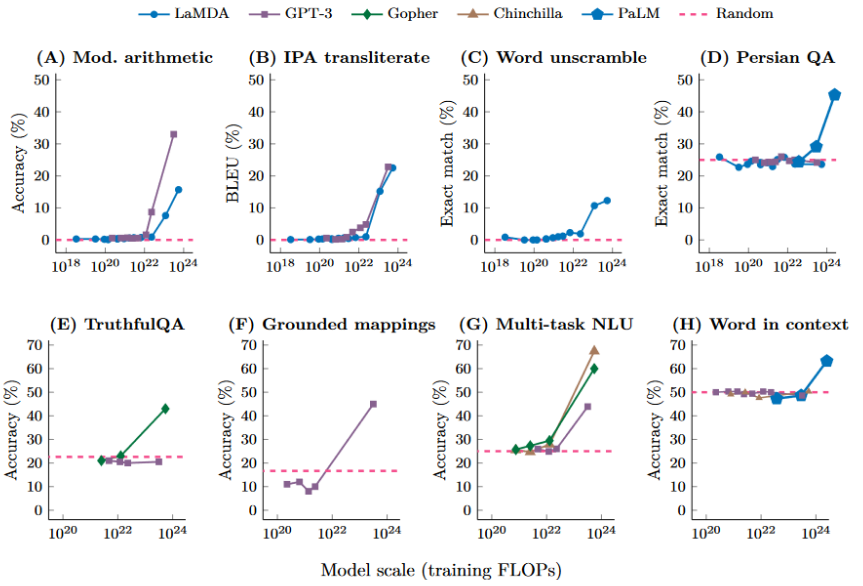
\includegraphics[width=0.84\textwidth]{figure/emergent_abilities.png}
    \caption{Examples of emergence in few-shot prompting. \citebutton{Wei et al., 2022}{https://arxiv.org/abs/2206.07682}}
    \label{fig:emergent_abilities}
\end{figure}

\vfill

\end{vbframe}

% ------------------------------------------------------------------------------

\begin{vbframe}{Emergent tasks in Big-Bench}

\vfill

\begin{itemize}
\item ``MODEL SIZE (TASK)'' means: MODEL can do
TASK with SIZE, but not with less than SIZE (hence emerging)
    \item GPT-3 13B (2 tasks): hindu knowledge, modified arithmetic
    \item GPT-3 175B (15 tasks): analytic entailment, codenames, phrase relatedness, question answer creation, self evaluation tutoring, ...
    \item LaMDA 137B (8 tasks): gender inclusive sentences german, repeat copy logic, sports understanding, ...
    \item PaLM 8B (3 tasks): auto debugging, sufficient information, ParsiNLU reading comprehension
    \item PaLM 64B (14 tasks): anachronisms, ascii word recognition, conceptual combinations, ...
    \item PaLM 540B (25 tasks): analogical similarity, causal judgment, code line description, crass ai, cs algorithms, ...
\end{itemize}

\vfill

\end{vbframe}

% ------------------------------------------------------------------------------

\begin{vbframe}{Emergent tasks in MMLU}

\vfill

\begin{itemize}
    \item Chinchilla 7B (7 tasks): Professional Medicine, High School Statistics, High School Macroeconomics, High School Psychology, Anatomy, High School Government And Politics, High School Microeconomics
    \item Chinchilla 70B (44 tasks): International Law, Human Aging, Sociology, Us Foreign Policy, High School World History, Marketing, Logical Fallacies, Miscellaneous, College Biology, High School Us History, Security Studies, High School European History, ...
\end{itemize}

\vfill

\end{vbframe}

% ------------------------------------------------------------------------------

\begin{vbframe}{Other emergent tasks}

\vfill

\begin{itemize}
    \item GPT-3 paper: 3 digit addition/subtraction (GPT-3 13B), 4-5 digit addition/substraction (GPT-3 175B), leveraging few-shot examples for word denoising (GPT-3 13B)
    \item Gopher paper: Toxicity classification (Gopher 7.1B), TruthfulQA (Gopher 280B)
    \item Patel \& Pavlick: grounded conceptual mappings (GPT-3 175B)
    \item PaLM paper: Word in Context benchmark (PaLM 540B)
\end{itemize}

\vfill

\end{vbframe}

% ------------------------------------------------------------------------------

% \begin{vbframe}{Impact of Model Size}

% \vfill

% \vfill

% \end{vbframe}

% ------------------------------------------------------------------------------

\begin{vbframe}{counter argument}

\citebutton{Source: Schaeffer et al., 2023}{https://arxiv.org/pdf/2304.15004.pdf}

\vfill

Two defining properties for emergent abilities in LLMs:

\begin{enumerate}
%
\item \textbf{Sharpness:} transitioning seemingly instantaneously from not present to present
%
\item \textbf{Unpredictability:} transitioning at seemingly unforeseeable model scales
%
\end{enumerate}

\vskip5mm

Claim: Emergent abilities appear only under metrics that nonlinearly or discontinuously scale model's per-token error rate:

	\begin{figure}
		\centering
		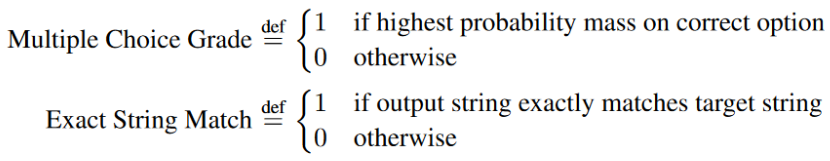
\includegraphics[width = 11cm]{figure/metrics.png} \\ 
	\end{figure}

\vfill

\end{vbframe}

% -----------------------------------------------------------------------------

\begin{vbframe}{counter argument}

\vfill

	\begin{figure}
		\centering
		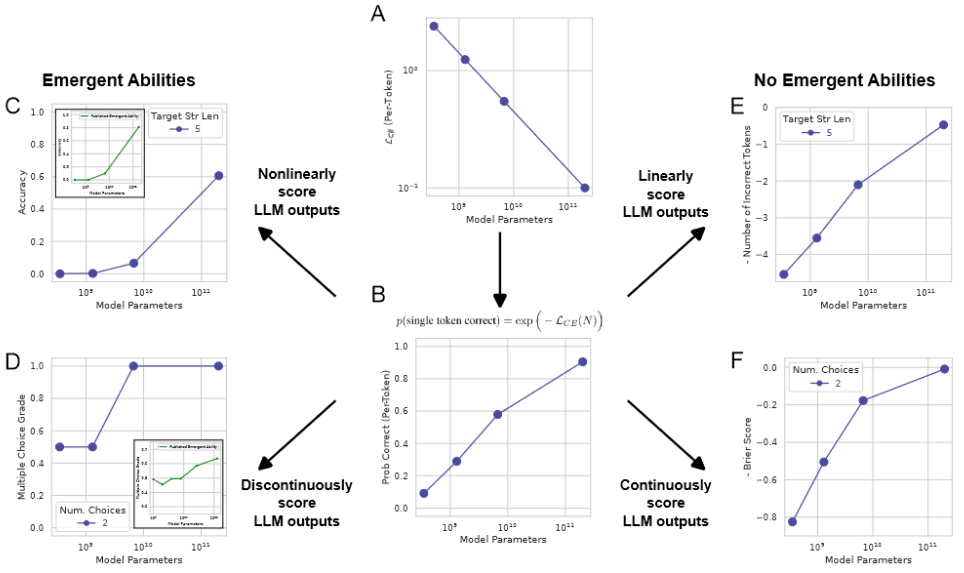
\includegraphics[width = 11cm]{figure/emergent_experiments.png}\\ 
		\citebutton{Source: Schaeffer et al., 2023}{https://arxiv.org/pdf/2304.15004.pdf}
	\end{figure}

\vfill

\end{vbframe}

% ------------------------------------------------------------------------------

\begin{vbframe}{Counterargument: Summary}

\vfill

%\textbf{Conclusions:}
%
\begin{itemize}
%
\item
If TASK is emergent for family MODEL at SIZE on METRIC, then
it is often possible to choose another metric for which the
task is not emergent.
%
\item Emergent abilities can be induced in computer vision tasks as well
%
\item A task and a metric are distinct and meaningful choices when constructing a benchmark
%
\item When choosing a metric, one should consider the
metric's effect on the per-token error rate;
may require adapting the measuring process
%
\end{itemize}


\vfill

\end{vbframe}

% ------------------------------------------------------------------------------

% ------------------------------------------------------------------------------

\begin{vbframe}{counter counter argument}

\vfill

%
\begin{itemize}
\item \ques What was your emergence moment with LLMs?
%\item Subjectively, there was clearly some form of ``psychological'' emergence
%when GPT3 and InstructGPT came out (several other models
%as well)

%
\end{itemize}


\vfill

\end{vbframe}

\begin{vbframe}{Back to finetuning}

\vfill

%
\begin{itemize}
\item \ques You are working at a telecommunications
company. You are given the task of converting a German manual from
polite form (``Wir sind jederzeit unter der folgenden
Nummer fuer Sie erreichbar'') to familiar form
(``Wir sind jederzeit unter der folgenden
Nummer fuer Dich erreichbar''). How would you do this?

\end{itemize}


\vfill

\end{vbframe}


% ------------------------------------------------------------------------------

% \begin{vbframe}{Summary}

% \vfill

% \begin{itemize}
%     \item Can we improve model architectures?
%     \item Can we improve data quality and quantity? 
%     \item Better prompting.
%     \item Frontier tasks. 
%     \item Why do emergent abilities occur, and can we predict them? 
% \end{itemize}

% \vfill

% \end{vbframe}

% ------------------------------------------------------------------------------

\endlecture
\end{document}
